\chapter{Week}
In this week a more closer evaluation of available neural network inference tools by Intel was done. The reason for this is the dependency solely on one \ac{FPGA} supplier is not ideal. In order to be flexible with product design and familiarity with all of the tools on the market for neural network inference, it was decided that some time should be spend on evaluating alternatives to Xilinx.
\begin{figure}[!htb]
	\centering
		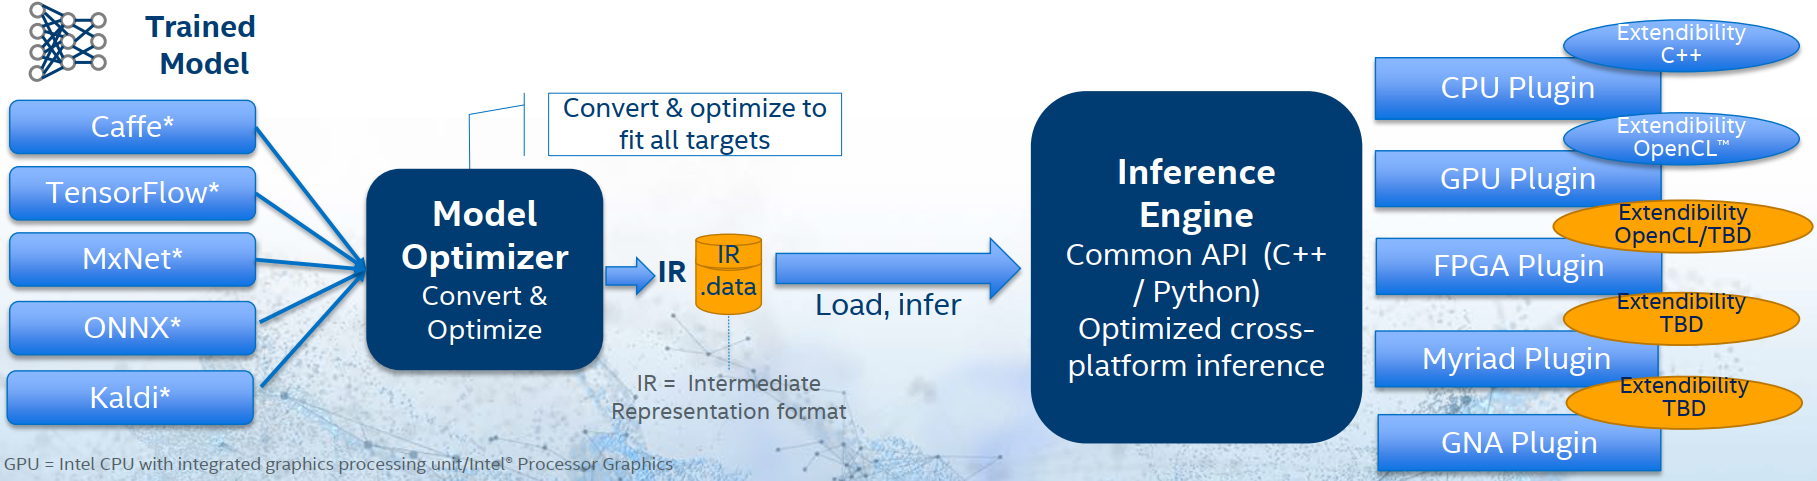
\includegraphics[width=\textwidth]{bilder/openVINO-overview.png}
		\caption{OpenVINO toolkit overview~\cite{openvino}}
		\label{fig:openvino}
\end{figure}
Figure~\ref{fig:openvino} shows an overview over Intels OpenVINO toolkit. The workflow itself is similar to Xilinx \ac{DNNDK}. The starting point is a trained model using popular neural network training frameworks (Caffe, Tensorflow, etc.). The trained network is then passed to a model optimizer which performs tasks such as quantization, stripping away layers only needed for training and other tasks. This operation is hardware independent. An intermediate representation is generated and passed on to the inference engine. This is a high level \ac{API} allowing the implementation of neural networks on the target hardware. The main difference is its universal approach compared to the Xilinx \ac{DNNDK}. Intel acquired the \ac{FPGA} company Altera and took over their \ac{FPGA} modules. Therefore, the OpenVINO toolkit does not only support \acp{FPGA} but also all of other product families Intel offers, such as \acp{CPU}, \acp{GPU} as well as other more specialized hardware. One of the main problems with Intels offering is its support of only one \ac{FPGA} familiy, namely the Arria 10 \acp{FPGA}. Moreover, the model optimizer is not as powerful as the Xilinx \ac{DNNDK} one. No pruning is taking place and as of this date, there is no support for INT8 precision, only reduced precision floating point, which is not ideal. Therefore, the Xilinx approach is deemed superior.
Integration and building of a custom Petalinux distribution continued this week with familiarizing myself with the overall workflow and possible debugging features. The \ac{DPU} \ac{IP} core was successfully integrated into the ZCU 104 reference design and synthesized. As the \ac{DNNDK} tool is still in a beta phase, there are frequent updates. A major update was released this week. This updated version was investigated and documented in the internal Enclustra Wiki. New sample applications were tested with the ZCU 104 evaluation board.